\documentclass[%
	%draft
	]{ijsra}
\def\IJSRAidentifier{\currfilebase} %<---- don’t change this!
%-------Title | Email | Keywords | Abstract-------------
\def\shorttitle{Gods, Games, and Geography}
\def\maintitle{Gods, Games, and Geography: A Cross Cultural Study of Chance Games and Religious Ideology}
\def\cmail{ddavis17@binghamton.edu}
\def\keywords{cross-cultural studies, anthropology, games of chance, religion, geography, spatial analysis}
%\def\keywordname{}%<--- redefine the name “Keywords“ in needed language
\def\abstract{Previously, cross-cultural studies have been limited by an immense, but largely inaccessible, volume of literature, most of which was not easily comparable to other studies. Recently, with the advent of D-PLACE (a global database of cultural, linguistic, and environmental data), cross-cultural analyses can be conducted between over 1400 different cultural groups with relative ease. Utilising this new database, a re-examination of the revolutionary article by Roberts and colleagues, \textit{Games in Culture} (1959) is undertaken, specifically to address the hypothesis that games of chance are more prevalent in cultural groups with “benevolent” gods. Additionally, variables of political integration, mean community population size, geographic location, and the belief in trance states and possession are incorporated to explore correlations between game type presence and religious differences. A total of 377 different cultures are compared in this study, making this the largest sample size used to re-evaluate the \textit{Games in Culture} hypotheses. Games are abundant in the archaeological record, and provide much detail regarding cultural, religious, and social characteristics of different groups. Thus, this study not only holds anthropological merit, but also benefits the archaeological community.}
%--------Author’s names------------
\def\authorone{Dylan Davis}
%-------Biographical information-------------
\def\bioone{ ...}
%------University/Institution--------------
\def\affilone{Binghamton University}

\begin{filecontents}{\IJSRAidentifier.bib}

@ARTICLE {ball1972,
	author  = "Ball, Donald W",
	title   = "The Scaling of Gaming: Skill, Strategy, and Chance",
	journal = "The Pacific Sociological Review",
	year    = "1972",
	volume  = "15",
	number  = "3",
	pages   = "277-294"
}

@ARTICLE {barry1980,
	author  = "Barry, Herbert",
	title   = "Ethnographic Atlas XXVIII",
	journal = "Ethnology",
	year    = "1980",
	volume  = "19",
	number  = "2",
	pages   = "245-263"
}

@BOOK {bell1992,
	author    = "Bell, Catherine",
	title     = "Ritual theory, ritual practice",
	publisher = "Oxford University Press",
	year      = "1992",
	location   = "New York"
}

@ARTICLE {binde2005,
	author  = "Binde, Per",
	title   = "Gambling Across Cultures: Mapping Worldwide Occurrence and Learning from Ethnographic Comparison",
	journal = "International Gambling Studies",
	year    = "2005",
	volume  = "5",
	number  = "1",
	pages   = "1–27"
}

@ARTICLE {binde2007,
	author  = "Binde, Per",
	title   = "Gambling and religion: Histories of concord and conflict",
	journal = "Journal of Gambling Issues",
	year    = "2007",
	volume  = "20",
	pages   = "145-165"
}

@ARTICLE {bondarenko2005,
	author  = "Bondarenko, Dmitri, Alexander Kazankov, Daria Khaltourina, and Andrey Korotayev",
	title   = "Ethnographic atlas XXXI: Peoples of easternmost Europe",
	journal = "Ethnology",
	year    = "2005",
	volume  = "44",
	number  = "3",
	pages   = "261-289"
}

@ARTICLE {botero2014,
	author  = "Botero, Carlos A., Beth Gardner, Kathryn R. Kirby, Joseph Bulbulia, Michael C. Gavin, and Russell D. Gray",
	title   = "The ecology of religious beliefs",
	journal = "Proceedings of the National Academy of Sciences",
	year    = "2014",
	volume  = "111",
	number  = "47",
	pages   = "16784-16789"
}

@ARTICLE {chick1984,
	author  = "Chick, Garry E",
	title   = "The Cross-Cultural Study of Games",
	journal = "Exercise and Sport Sciences Reviews",
	year    = "1984",
	volume  = "12",
	pages   = "307-337"
}

@ARTICLE {chick1998,
	author  = "Chick, Garry",
	title   = "Games in Culture Revisited: A Replication and Extension of Roberts, Arth, and Bush (1959)",
	journal = "Cross-Cultural Research",
	year    = "1998",
	volume  = "32",
	number  = "2",
	pages   = "185-206"
}

@INCOLLECTION {chick2015,
	author    = "Chick, Gary",
	title     = "Games and Sports",
	booktitle = "Explaining Human Culture",
	publisher = "Human Relations Area Files",
	year      = "2015",
	editor    = "C. R. Ember",
	pages     = "Accessed July 14, 2016. http://hraf.yale.edu/ehc/summaries/ games-and-sports"
}

@ARTICLE {crist2016,
	author  = "Crist, Walter, Alex de Voogt, and Anne-Elizabeth Dunn-Vaturi",
	title   = "Facilitating Interaction: Board Games as Social Lubricants in the Ancient Near East.",
	journal = "Oxford Journal of Archaeology",
	year    = "2016",
	volume  = "35",
	number  = "2",
	pages   = "179–196"
}

@ARTICLE {davis,
	author  = "Davis, Dylan S.",
	title   = "The Power of Ideology: Religion and Environmental Sustainability in Prehistoric Societies",
	journal = "Nexus: The Canadian Student Journal of Anthropology",
	year    = "In Press",
	volume  = "24",
	number  = "1"
}

@ARTICLE {devoogt2013,
	author  = "de Voogt, Alex, Anne-Elizabeth Dunn-Vaturi, and Jelmer W. Eerkens",
	title   = "Cultural transmission in the ancient Near East: twenty squares and fifty-eight holes",
	journal = "Journal of Archaeological Science",
	year    = "2013",
	volume  = "40",
	number  = "4",
	pages   = "1715-1730"
}

@ARTICLE {deaner2012,
	author  = "Deaner, Robert O., and Brandt A. Smith",
	title   = "Sex Differences in Sports Across 50 Societies",
	journal = "Cross-Cultural Research",
	year    = "2012",
	volume  = "47",
	number  = "3",
	pages   = "268–309"
}

@STANDARD {D-PLACE,
	title    = "About D-PLACE – the Database of Places, Language, Culture and Environment",
	author   = "D-PLACE",
	revision = "Accessed July 15, 2016",
	year     = "2016",
	url      = "https://d-place.org/about"
}

@ARTICLE {fast2009,
	author  = "Fast, Nathanael J., Deborah H Gruenfeld, Niro Sivanathan, and Adam D. Galinsky",
	title   = "Illusory Control : A Generative Force Behind Power's Far-Reaching Effects",
	journal = "Psychological Science",
	year    = "2009",
	volume  = "20",
	number  = "4",
	pages   = "502-508"
}

@BOOK {faulkner2008,
	author    = "Faulkner, Raymond, Ogden Goelet, Carol Andrews, and James Wasserman",
	title     = "The Egyptian Book of the Dead: The Book of Going Forth by Day-The Complete Papyrus of Ani Featuring Integrated Text and Full-Color Images",
	publisher = "Chronicle Books",
	year      = "2008",
	location   = "San Francisco"
}

@INCOLLECTION {finkel1990,
	author    = "Finkel, Irving L.",
	title     = "On the Rules for the Royal Game of Ur.",
	booktitle = "Ancient Board Games in Perspective: Papers from the 1990 British Museum Colloquium, with Additional Contributions",
	publisher = "British Museum",
	year      = "2007",
	editor    = "I.L. Finkel",
	pages     = "16-32",
	location   = "London"
}

@BOOK {gobet2004,
	author    = "Gobet, Fernand, Jean Retschitzki, and Alex de Voogt",
	title     = "Moves in mind: The psychology of board games",
	publisher = "Psychology Press",
	year      = "2004",
	location   = "New York"
}

@INCOLLECTION {gosso2005,
	author    = "Gosso, Yumi, Emma Otta, Maria de Lima Salum e Morais, Fernando José Leite Ribeiro, and Vera Silvia Raad Bussab",
	title     = "Play in Hunter-Gatherer Society",
	booktitle = "The Nature of Play: The Great Apes and Humans",
	publisher = "Guilford Press",
	year      = "2005",
	editor    = "Anthony D. Pellegrini and Peter K. Smith",
	pages     = "213-254",
	location   = "New York"
}

@ARTICLE {gray1999,
	author  = "Gray, J. Patrick",
	title   = "A corrected ethnographic atlas",
	journal = "World Cultures",
	year    = "1999",
	volume  = "10",
	number  = "1",
	pages   = "24–85"
}

@ARTICLE {hall2016,
	author  = "Hall, Mark A.",
	title   = "Board Games in Boat Burials: Play in the Performance of Migration and Viking Age Mortuary Practice",
	journal = "European Journal of Archaeology",
	year    = "2016",
	volume  = "19",
	number  = "3",
	pages   = "439-455"
}

@ONLINE {hodder2016,
	author = "Hodder, Ian.",
	title  = "Studies in Human-Thing Entanglement",
	month  = "mar",
	year   = "2016",
	url    = "http://www.ian-hodder.com/books/studies-human-thing-entanglement"
}

@INCOLLECTION {kendall2007,
	author    = "Kendall, Timothy",
	title     = "Mehen: the ancient Egyptian game of the serpent",
	booktitle = "Board Games in Perspective: Papers from the 1990 British Museum Colloquium, with Additional Contributions",
	publisher = "British Museum Press",
	year      = "2007",
	editor    = "I. Finkel",
	pages     = "33-45",
	location   = "London"
}

@ARTICLE {kirby2016,
	author  = "Kirby, K.R., R.D. Gray, S.J. Greenhill, F.M. Jordan, S. Gomes-Ng, H.J. Bibiko, D.E. Blasi, et al.",
	title   = "D-PLACE: A Global Database of Cultural, Linguistic and Environmental Diversity",
	journal = "PLoS ONE",
	year    = "2016",
	volume  = "11",
	number  = "7",
	pages   = "e0158391"
}

@ARTICLE {korotayev2004,
	author  = "Korotayev, Andrey, Alexander Kazankov, Svetlana Borinskaya, Daria Khaltourina, and Dmitri Bondarenko",
	title   = "Ethnographic atlas XXX: peoples of Siberia",
	journal = "Ethnology",
	year    = "2004",
	volume  = "43",
	number  = "1",
	pages   = "83–92"
}

@ARTICLE {lambert1959,
	author  = "Lambert, William W., Leigh Minturn Triandis, and Margery Wolf",
	title   = "Some correlates of beliefs in the malevolence and benevolence of supernatural beings: A cross-societal study",
	journal = "The Journal of Abnormal and Social Psychology",
	year    = "1959",
	volume  = "58",
	number  = "2",
	pages   = "162-169"
}

@ARTICLE {langer1975,
	author  = "Langer, E. J.",
	title   = "The illusion of control",
	journal = "Journal of personality and social psychology",
	year    = "1975",
	volume  = "31",
	number  = "2",
	pages   = "311-328."
}

@ARTICLE {lansing1993,
	author  = "Lansing, J. Stephen, and James N. Kremer",
	title   = "Emergent Properties of Balinese Water Temple Networks: Coadaptation on a Rugged Fitness.",
	journal = "American Anthropologist",
	year    = "1993",
	volume  = "95",
	number  = "1",
	pages   = "97-114"
}

@ARTICLE {murdock1962,
	author  = "Murdock, George Peter",
	title   = "Ethnographic Atlas, Installments I-XXVII",
	journal = "Ethnology",
	year    = "1962-1971",
	volume  = "1-10"
}

@ARTICLE {murdock1957,
	author  = "Murdock, George Peter",
	title   = "World Ethnographic Sample",
	journal = "American Anthropologist",
	year    = "1957",
	volume  = "59",
	number  = "4",
	pages   = "664-687"
}

@ARTICLE {peregrine2008,
	author  = "Peregrine, Peter N.",
	title   = "Political Strategy and Cross-Cultural Variation in Games",
	journal = "Cross-Cultural Research",
	year    = "2008",
	volume  = "42",
	number  = "4",
	pages   = "386–393"
}

@ARTICLE {piccione1980,
	author  = "Piccione, Peter A.",
	title   = "In search of the meaning of Senet In Archaeology",
	journal = "Archaeology",
	year    = "1980",
	volume  = "33",
	pages   = "55-58"
}

@INCOLLECTION {piccione2007,
	author    = "Piccione, Peter A.",
	title     = "The Egyptian Game of Senet and the Migration of the Soul",
	booktitle = "Ancient Board Games in Perspective: Papers from the 1990 British Museum Colloquium, with Additional Contributions",
	publisher = "British Museum Press",
	year      = "2007",
	editor    = "I. Finkel",
	pages     = "54-63",
	location   = "London"
}

@INCOLLECTION {purzycki2011,
	author    = "Purzycki, Benjamin G., and Richard Sosis",
	title     = "Our Gods: Variation in Supernatural Minds",
	booktitle = "Essential Building Blocks of Human Nature",
	publisher = "Springer-Verlag",
	year      = "2011",
	editor    = "Ulrich J. Frey, Charlotte Störmer and Kai P. Willführ",
	pages     = "77-93",
	location   = "New York"
}

@ARTICLE {purzycki2013,
	author  = "Purzycki, Benjamin Grant",
	title   = "The minds of gods: A comparative study of supernatural agency",
	journal = "Cognition",
	year    = "2013",
	volume  = "129",
	number  = "1",
	pages   = "163-179"
}

@ARTICLE {purzycki2016,
	author  = "Purzycki, Benjamin Grant, Coren Apicella, Quentin D. Atkinson, Emma Cohen, Rita Anne McNamara, Aiyana K. Willard, Dimitris Xygalatas, Ara Norenzayan, and Joseph Henrich",
	title   = "Moralistic gods, supernatural punishment and the expansion of human sociality",
	journal = "Nature",
	year    = "2016",
	volume  = "530",
	pages   = "327–330"
}

@ARTICLE {roberts1959,
	author  = "Roberts, John M., Malcolm J. Arth, and Robert R. Bush",
	title   = "Games in Culture",
	journal = "American Anthropologist",
	year    = "1959",
	volume  = "61",
	number  = "4",
	pages   = "597-605"
}

@STANDARD {robinson2015,
	title       = "Social ritual and religion in ancient Egyptian board games",
	institution = "Museum of Gaming Research Centre",
	author      = "Robinson, Phillip",
	year        = "2015",
	url         = "http://www.museumofgaming.org.uk/papers/ritual_in_egyptian_board_games.pdf",
	note        = "Accessed July 28, 2016"
}

@ARTICLE {rogersdotter2015,
	author  = "Rogersdotter, Elke",
	title   = "What’s Left of Games are Boards Alone: on Form, Incidence, and Variability of Engraved Game Boards at Vijayanagara (c. AD 1350-1565)",
	journal = "Heritage: Journal of Multidisciplinary Studies in Archaeology",
	year    = "2015",
	volume  = "3",
	pages   = "457-496"
}

@ARTICLE {sipes1973,
	author  = "Sipes, Richard G.",
	title   = "War, Sports and Aggression: An Empirical Test of Two Rival Theories",
	journal = "American Anthropologist",
	year    = "1973",
	volume  = "75",
	number  = "1",
	pages   = "64-86"
}

@ARTICLE {stevenson1903,
	author  = "Stevenson, Matilda Coxe",
	title   = "Zuñi Games",
	journal = "American Anthropologist",
	year    = "1903",
	volume  = "5",
	number  = "3",
	pages   = "468-497"
}

@ARTICLE {tobacyk1991,
	author  = "Tobacyk, Jerome J., and Lamar V. Wilkinson",
	title   = "Paranormal beliefs and preference for games of chance",
	journal = "Psychological Reports",
	year    = "1991",
	volume  = "68",
	number  = "3 suppl",
	pages   = "1088-1090"
}

@ARTICLE {wohl2002,
	author  = "Wohl, Michael J. A., and Michael E. Enzle",
	title   = "The Deployment of Personal Luck: Sympathetic Magic and Illusory Control in Games of Pure Chance.",
	journal = "Personality and Social Psychology Bulletin",
	year    = "2002",
	volume  = "28",
	number  = "10",
	pages   = "1388-1397"
}
\end{filecontents}

\begin{document}
\IJSRAopening%<---- don’t change this!
%-------
%(A) Appendix??;
%(B) embedded quotes??;
%(C) Citations in abstract??

\lettrine{A}{mong} the various sub-disciplines of anthropology, the anthropology of games and recreation is one such subfield that has remained under the radar, attracting only a small number of scholars for the past century. However, there are many important relationships that exist between gameplay and various cultural characteristics, including a link between strategy games and socio-political organisation \parencite[see][]{peregrine2008}. Additionally, the presence of combat sports has been correlated with increased levels of warfare in human groups \parencites[8]{chick2015}{sipes1973}. Different game types are spread unevenly throughout the world \parencites[309]{chick1984}{chick2015}{roberts1959}, and as such, the presence of some game types can signify certain components of a group of people. Furthermore, it has been suggested that the types of games (and number of different games) that are present within a given society are related to the overall complexity of that society \parencites[313]{chick1984}{roberts1959}.

Recreational activities are, for the most part, invisible in the archaeological record. For example, rough and tumble play (e.g. wrestling), fantasy play (e.g. roleplaying), and social contingency play (e.g. some form of play that attempt to instil pleasure in others, such as imitation), which do not require the use of objects may not leave archaeologically visible evidence \parencite[218-19]{gosso2005}. However, games that utilise objects (e.g. weapons, game boards/pieces, etc.) that will preserve in the archaeological record can reveal a great deal about past cultural groups. For example, a study of Middle-Eastern board-games (i.e. \textit{senet} and \textit{mehen}) provides evidence that such games encouraged social interactions between social classes \parencite{crist2016}. In addition to social interactions, board-games have also been used for divination \parencite[25]{finkle2007} and have been found in association with burials \parencite[440]{hall2016}.

The presence of material remains of games (e.g. boards of board-games, dice, etc.) can reveal important information about different human groups, both in terms of their sociality as well as their political and religious beliefs. For instance, the game of \textit{senet}, which began as a strictly secular pastime, acquired religious significance over time throughout the history of Ancient Egypt \parencite{piccione1980}.  The game, which is more a ``game of chase” rather than one of strategy \parencite{faulkner2008} consists of a board with 30 squares over which pieces are moved. The game became entangled with religious views of the life after death in ancient Egypt \parencite{piccione1980} and was transformed into ``an allegory of the afterlife” \parencite[158]{faulkner2008}. The presence of game pieces in archaeological material culture can also hint at geographical extents of certain empires or societal groups \parencite[1717]{devoogt2013} as well as the spread of ideas.

Among the most intriguing questions pertaining to the anthropology of games is related to the presence of games of chance and their relationship to religious ideology. This relationship was first mentioned by \textcite{richards1959} in their seminal article \textit{Games in Culture}. This correlation was made utilising a small sample of cultural groups ($n = 20$) and was not able to be replicated by later studies \parencite[e.g.][]{chick1998}. It is the goal of this paper to retest the hypotheses of Richards and colleagues (1959) relating to games of chance and religious beliefs. In addition to using a larger sample of cultural groups and additional variables of religious variation, alternate factors will also be explored including geographic location and population size to address why games of chance only occur in certain regions. This will provide important insight not only for anthropologists, but archaeologists as well, especially in terms of cultural significance that is not as easily attainable from the archaeological record.

\IJSRAsection{A Revisitation of Roberts and Colleagues (1959)}

In their article, \textit{Games in Culture}, Roberts et al. (1959) establish several hypotheses about the nature of game types across different cultures around the world. Among their various conclusions are:

\begin{enumerate}
\item Games of strategy are correlated with social systems and hierarchical complexity;
\item Games of chance are correlated with religion, and;
\item Games of physical skill are potentially related to environmental conditions \parencite[604]{roberts1959}.
\end{enumerate}

In a re-visitation of the study by \textcite{chick1998}, most of the hypotheses developed by Roberts and colleagues are upheld. However, one hypothesis regarding religion and its correlation with the presence of games of chance was unable to be confirmed by \textcite[192]{chick1998}; namely that games of chance are associated with the presence of ``benevolent” gods. Utilising data from D-BASE and the Ethnographic Atlas \parencites{murdock1962}{barry1980}{gray1999}{korotayev2004}{bondarenko2005}, an investigation into the validity of the religion/chance hypothesis of \textcite{roberts1959} is undertaken.

In their 1959 article, \textcite{roberts1959} examine 20 different cultural groups out of 62 different cultures detailed in a study by \textcite{lambert1959}. The basic hypothesis of \textcite[601-602]{roberts1959} is that games of chance are linked – and therefore appear in greater numbers – in cultural groups with strong religious beliefs in the supernatural, and furthermore, that such games of chance serve as a means to explore the relationship between humans and supernatural beings. Specifically, Roberts et al. state that games of chance will be more frequent in groups with benevolent or coercive gods, and less frequent in groups with aggressive gods. The results of their study support their hypotheses (see \cref{fig:Davis-Table01}). However, using only a total of 20 different cultures\footnote{Although two studies utilise 19 cultural groups and the third uses 15, there are overlaps between all of the hypotheses and a total of 20 different cultural groups are used.} leads to some concerns about the validity of the results. Especially with \textcite{chick1998} not being able to replicate the results (due to a lack of availability of data), it is important to revisit this conclusion.
 
 	\begin{figure}[!htb] %TABLE 1
 		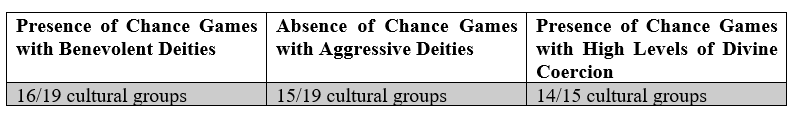
\includegraphics[width=\linewidth]{figures/Davis-Table01}
 		\captionof{table}{Results of Roberts \textit{et al.} (1959) study}
 		\centering
 		\label{fig:Davis-Table01}
 	\end{figure}
 
 \IJSRAsection{D-PLACE}
 
 Comparisons between world cultures can provide important insights into human nature and general societal patterns. In the past, comparison was often limited to a small number of case studies within most literature. Now, however, with the advent of D-PLACE ()\url{http://d-place.org} – an open access database of global cultures, linguistic patterns, and environmental diversity – comparisons between different human groups can be conducted between over 1400 different ‘societies’ \parencite{kirby2016}. A ‘society’ is defined by the D-PLACE database as ``a group of people in a particular locality, who often share a language and cultural identity” \parencite{D-PLACE}. In order to keep terminology as homogeneous as possible, I will refer to such groups as \textit{cultural groups} rather than societies, in order to avoid any confusion in mixing these terminologies.
 
 Utilising D-PLACE, examinations of cultural change, as well as correlations between cultural, linguistic, and environmental variables can be compared between a multitude of different groups \parencite{kirby2016}. By looking at several different variables at once across hundreds (if not thousands) of different cultural groups, many new discoveries can be made that were up until recently, practically impossible. For this study, the Ethnographic Atlas dataset was used, which contains information from over 90 different cultural traits \parencite{kirby2016}. One note on the Ethnographic Atlas data that is necessary to mention is that although it is a global dataset, there is an emphasis on North American and African cultural groups.
 
 When using D-PLACE, searches can be made by a culture group’s name, region(s) of interest, language family, cultural trait(s), or environmental variables. Up to four cultural traits and 3 environmental traits can be compared at one time. Once the desired variables are chosen, data can be visualised in a table, map, or phylogenic tree. Additionally, the data can be downloaded as a .csv file for further use. The most notable trait of D-PLACE is that it gathers a wealth of information and cultural data from a vast collection of literature and data repositories \parencite{kirby2016} that were previously either inaccessible, or extremely difficult to acquire and compare to other sources. This allows for greater scale cross-cultural comparison, and will enable future scholars to conduct studies that address long-time anthropological questions.

\IJSRAsection{Methods}

Using data from D-BASE, several different cultural and geographical comparisons were made addressing some three-hundred different cultural groups from around the world. The first of these comparisons aims at addressing the religious hypothesis of \textcite{roberts1959} and compares 377 different world cultures on the basis of two variables: the presence or absence of games of chance and the presence or absence of High Gods (See \cref{fig:Davis-Table04} in the Appendix).%%Appendix??
 In particular, the presence of ``moralistic” gods or deities that interact with humans was considered for this study. In order to link the presence or absence of ``moralistic” gods to benevolence or aggressiveness as discussed by \textcite{lambert1959} and \textcite{roberts1959}, the following information must be taken into consideration. 

When discussing ``morality” on a supernatural scale, the term refers to the concern a deity – or pantheon of deities – have about human social behaviours \parencite{purzycki2016}. ``Moralizing High Gods” are defined specifically as ``supernatural beings believed to have created or govern all reality, intervene in human affairs, and enforce or support human morality” \parencite[16784]{botero2014}. Furthermore, ``moralistic” gods promote cooperative behaviour while attempting to limit ``antisocial” behaviour \parencite[165]{purzycki2016}. When relating this definition to benevolence or aggressiveness, the following connection can be made: the presence of moralistic gods will contain supernatural beings who are concerned about humanity and will therefore be benevolent towards those who believe in said deity and conform to the values instilled by those gods. Conversely, however, moralistic gods also deliver punishment to those that disobey or fail to act in the manner expected or required by the god(s). As a result, both benevolence and aggressiveness are present within such a classification. On the other hand, in cultural groups without ``moralistic” gods, deities are either unconcerned with human affairs or are extremely distanced from humans, and therefore cannot be considered to be specifically benevolent or aggressive towards humanity. As discussed by \parencite[85]{purzycki2011}, ``[n]ot all supernatural agents, however, are concerned with the general moral behavior of people” and it has been shown using ecological modeling that religious traditions bound to local ecologies emphasise stress on sacrifice, especially in areas that require extensive resource management \parencite{lansing1993}. Cross-cultural analyses have shown that larger and more politically complex human-groups generally have a greater number of moralistic deities \parencite{purzycki2016}. Additionally, in areas that have ``High Gods” that are concerned with human morality, games tend to be more complex \parencite[290]{ball1972}. As a result, assuming the hypothesis of \textcite{roberts1959} is correct, if moralistic gods are present in a cultural group, games of chance should be more abundant. This is the first query of this paper (Q1).

Additional comparisons were conducted to address further correlations between game types, cultural differences, and geographical variables. Comparison was made between 54 cultures on the basis of game type, religious type, and the belief in trance states and possession (see \cref{fig:Davis-Table05} in the Appendix). Assuming that \textcite{roberts1959} is correct in their assumption that games of chance are more abundant in regions that exercise a belief in supernatural intervention, the belief in possession or divine intervention through trance states would be expected to have a statistical relationship with the presence or absence of games of chance (Q2). Comparison between 331 different cultures was also conducted on the basis of game type and mean community population size (see \cref{fig:Davis-Table06a} in the Appendix). Once again returning to \textcite{roberts1959}, assuming that the complexity of a cultural group is said to be correlated with the presence of strategy games and a greater number of different types of games altogether, the larger the population size, the greater the number of games that cultural group should have, including strategy games. Additionally, a look at political integration is explored in relation to the presence of strategy games (see \cref{fig:Davis-Table06b} in the Appendix), following the study of \textcite{roberts1959} (Q3). Finally, the same 377 cultural groups that were compared for Q1 were compared against their geographic positioning (latitude) in order to determine whether or not there is a geographic relationship to game types present in specific populations (Q4).\footnote{The different comparisons, although they contain different numbers of cultural groups, contain many overlaps and many of the cultures compared in one dataset are compared again in later data comparisons.} All of the tables depicting the list of cultures and their traits can be found in the Appendix of this article.

\IJSRAsection{Results}

\marginnote{Q1}

Of the 377 cultural groups sampled, 63 had games of chance present. Of these 63 populations, 53 of them also believed in a High God, many of which were ``moralistic” in nature. The other 10 did not believe in a High God that interacted with humans. Conducting a chi-squared test of independence ($n = 377$) revealed a statistically significant result ($\chi^{2} = 32.8, df = 1 p < 0.01$) indicating that a non-arbitrary correlation does exist between the presence of games of chance and the belief in High Gods. Relating the results back to \textcite{roberts1959}, 36 of the 53 cultures that had games of chance believed in a ``moralistic” god that directly intervened into human affairs. Such gods can be considered ``benevolent” – as described by \textcite{lambert1959} – in that they protect humans and instil morals to keep individuals in a state of peace. The other 17 cultural groups did not have ``moralistic” or benevolent gods and did have games of chance present. However, non-moral gods consisted of 128 cultural groups, whereas moralistic gods consisted of 65 cultural groups (see \cref{fig:Davis-Table02}). Statistical analysis of this data revealed that there is a statistically significant correlation between moralistic gods and the presence of games of chance ($n = 193, \chi^{2} = 38.4, df = 1, p < 0.01$).

\begin{figure}[!htb] %TABLE 2
	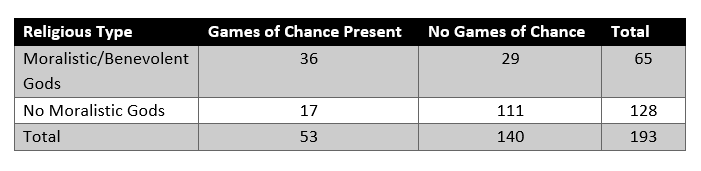
\includegraphics[width=\linewidth]{figures/Davis-Table02}
	\captionof{table}{}
	\centering
	\label{fig:Davis-Table02}
\end{figure}

\marginnote{Q2}

The second dataset compared trance states, religious type, and game type to test whether or not the belief in supernatural intervention was related to the presence of games of chance. The results disprove this hypothesis, as chi-square testing revealed statistically insignificant results, indicating that any correlation between these variables was likely due to chance ($n = 54, \chi^{2} = 6.77, df = 3, p > .05$).  When looking strictly at possession and excluding trance states, the results were even more independent, as the p-value was close to 0.8, indicating very little relativity between the presence of games of chance and belief in possession. These results do not necessarily mean that the belief in gods that intervene on a person’s behalf have no relevance to the abundance or scarcity of chance games, but statistically, the two variables are unrelated. This indicates that divination practices and the belief in supernatural possession of individuals or objects does not have any significant relationship with the presence of games of chance. However, as will be mentioned later, this does not mean that such beliefs are completely unrelated, as the belief in supernatural intervention in an indirect manner (e.g. fate, karma, etc.) is noticeable as a possible linkage with games of chance.

\marginnote{Q3}

331 different cultures were compared on the basis of game types present and their mean community population size (see \cref{fig:Davis-Table03} in the Appendix).\footnote{It will be noticed that not all culture groups have games. This is not to say that there was no recreational activity or game play of any kind, but rather speaks to the definition of games employed by the researchers and what activities were observed by ethnographers. D-PLACE adheres to the definition of games provided by \textcite{roberts1959} which specifies that ``games” must have an outcome with a winner and loser. As a result, if activities practiced by certain groups did not adhere to this criterion, then the activity would be regarded as recreational, but not a ``game.” Furthermore, if the ethnographers and anthropologists studying certain groups were uninterested in gameplay, then such information would be left out of their research. The way in which the term ``game” has been described by various researchers breeds ambiguity, and therefore, inconsistency within anthropology’s metalanguage is also partly responsible for a lack of data in some regions. This is one of the fundamental reasons as to why concise terminology is required for proper anthropological studies.} When visualising the data (see \cref{fig:Figure1_Davis_082016} and \cref{fig:Figure2_Davis_082016}) a correlation between game types and population size appears, with areas possessing more game types having larger population sizes. This pattern has been noticed by other researchers \parencites{ball1972}[322]{chick1984}[195]{chick1998}{roberts1959}. Overall, areas with larger mean community population sizes tend to have multiple game types present.

\begin{figure} [!htb] %FIGURE 1
	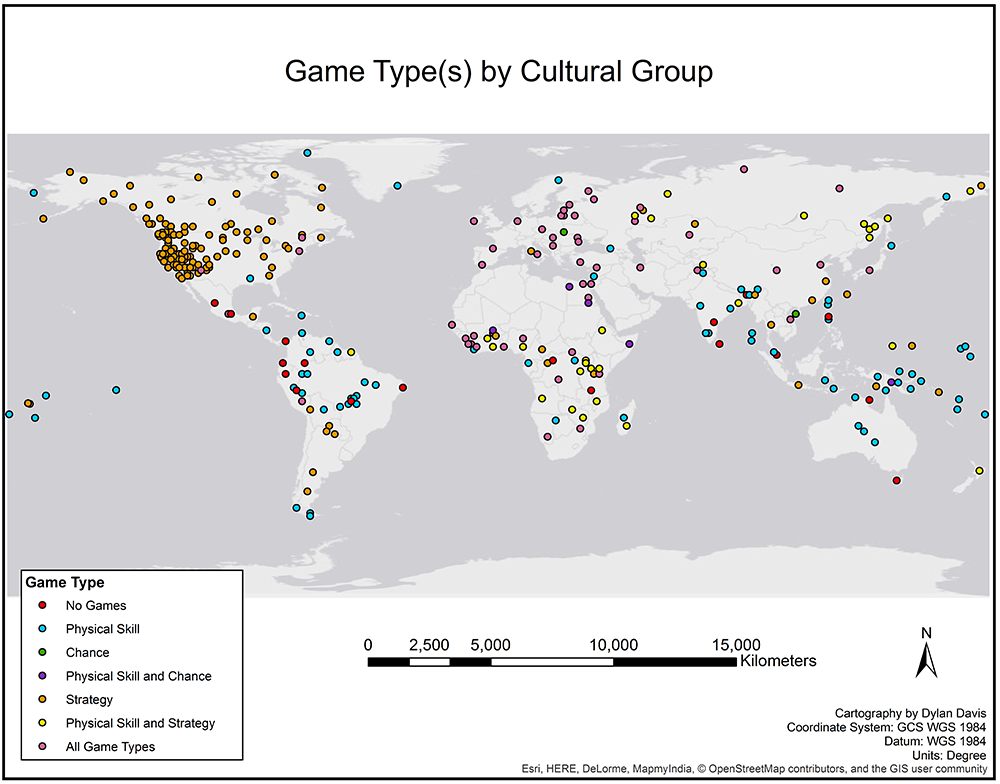
\includegraphics[width=\linewidth]{figures/Figure1_Davis_082016}
	\caption
	\centering
	\label{fig:Figure1_Davis_082016}
\end{figure}

\begin{figure} [!htb] %FIGURE 2
	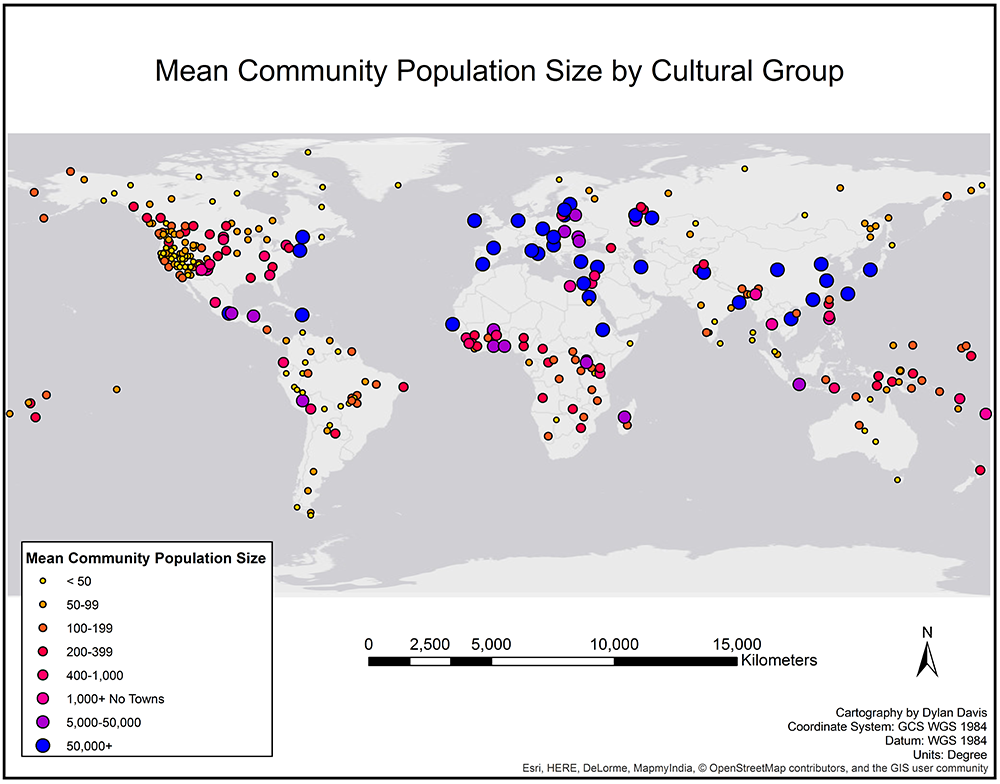
\includegraphics[width=\linewidth]{figures/Figure2_Davis_082016}
	\caption
	\centering
	\label{fig:Figure2_Davis_082016}
\end{figure}

In addition to comparing game types to mean community population size, a re-visitation of the study conducted by  \textcite{roberts1959} required a direct comparison of game types present in a cultural group to its level of political integration (see \cref{fig:Figure3_Davis_082016}).  \textcite{roberts1959} find that games of strategy are related to greater levels of hierarchical complexity and political integration. In their study, however, only 63 different cultural groups were compared. Utilising D-PLACE, 183 different cultural groups were compared on the basis of political complexity and whether or not games of strategy were present or absent.

\begin{figure} [!htb] %FIGURE 3
	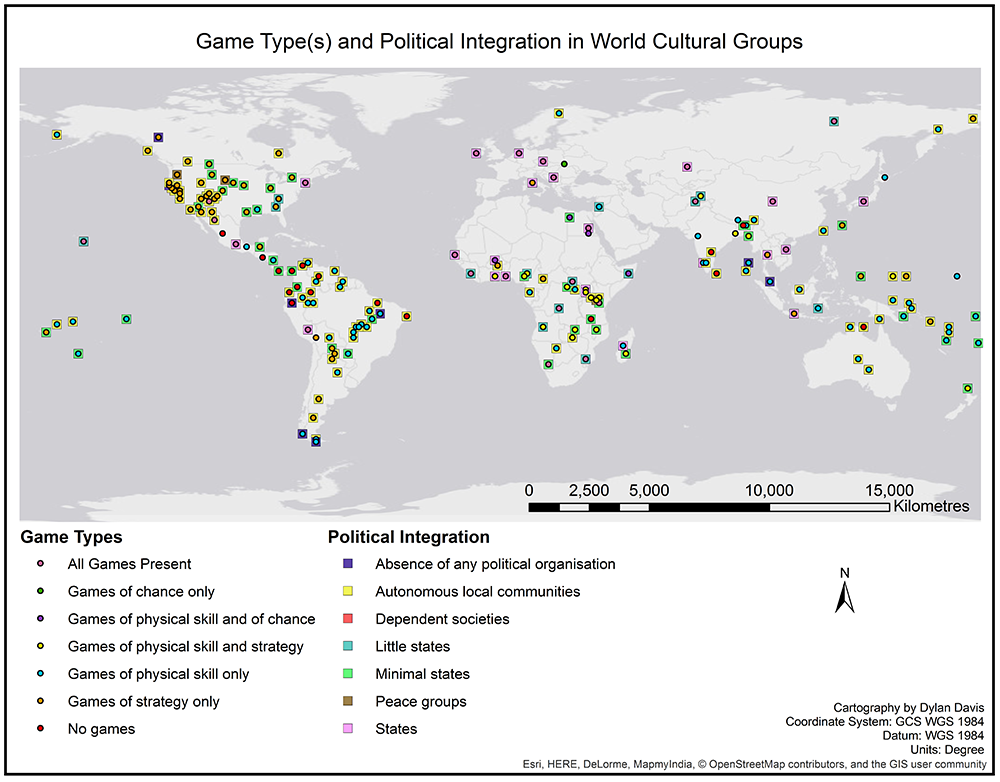
\includegraphics[width=\linewidth]{figures/Figure3_Davis_082016}
	\caption
	\centering
	\label{fig:Figure3_Davis_082016}
\end{figure}

Keeping with \textcite{roberts1959}, complex political organisation was determined on the basis of classifications established by \textcite{murdock1957}. As such the ratings of ``Autonomous Local Communities” and ``No Political Integration” as defined by \textcite{murdock1959} were considered to have ``low political integration” as established by \textcite{roberts1959}, and ``Minimal States”, ``Little States”, and ``States” were considered to have ``high political integration.” Additionally, populations that were classified as ``Absent”, ``Peace Groups”, or ``Dependent” by \textcite{murdock1957} were also considered to have ``low political integration” for this study. The results of a chi-square test of independence shows a high level of statistical significance ($\chi^{2} = 17.8, df = 1, p < 0.01$), indicating that \textcite{roberts1959} is correct in their hypothesis: games of strategy do have a statistical relationship with the level of political integration in a given cultural group.

\marginnote{Q4}

The last query of this paper examines if there are any geographic differences that relate to different game types that are present or absent in various cultural groups. The results are quite interesting. According to a cross-cultural analysis of the same 377 cultural groups examined for Q1, there is indeed a difference between latitudes and game types present, specifically games of chance (see \cref{fig:Davis-Table03} and \cref{fig:Figure4_Davis_082016}). As seen in the map and the table below, the overwhelming majority of cultural groups with games of chance present exist in the northern hemisphere, with 57 out of 63 (90.5\%) possessing games of chance existing in the northern hemisphere and only 6 out of 63 (9.5\%) existing in the southern hemisphere. Chi square tests reveal these results to be statistically significant ($\chi^{2} = 9.1, df = 1, p < 0.01$). These results were then compared to population sizes and religious types present and show relationships between these variables and geographical location. These results will be discussed in detail in the next section of this paper.

\begin{figure}[!htb] %TABLE 3
	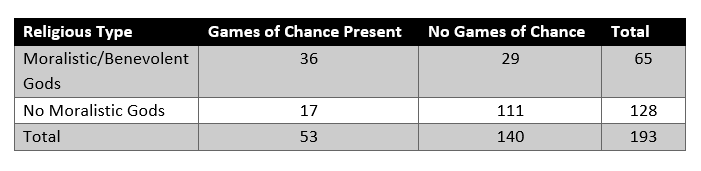
\includegraphics[width=\linewidth]{figures/Davis-Table02}
	\captionof{table}{}
	\centering
	\label{fig:Davis-Table03}
\end{figure}

\begin{figure} [!htb] %FIGURE 4
	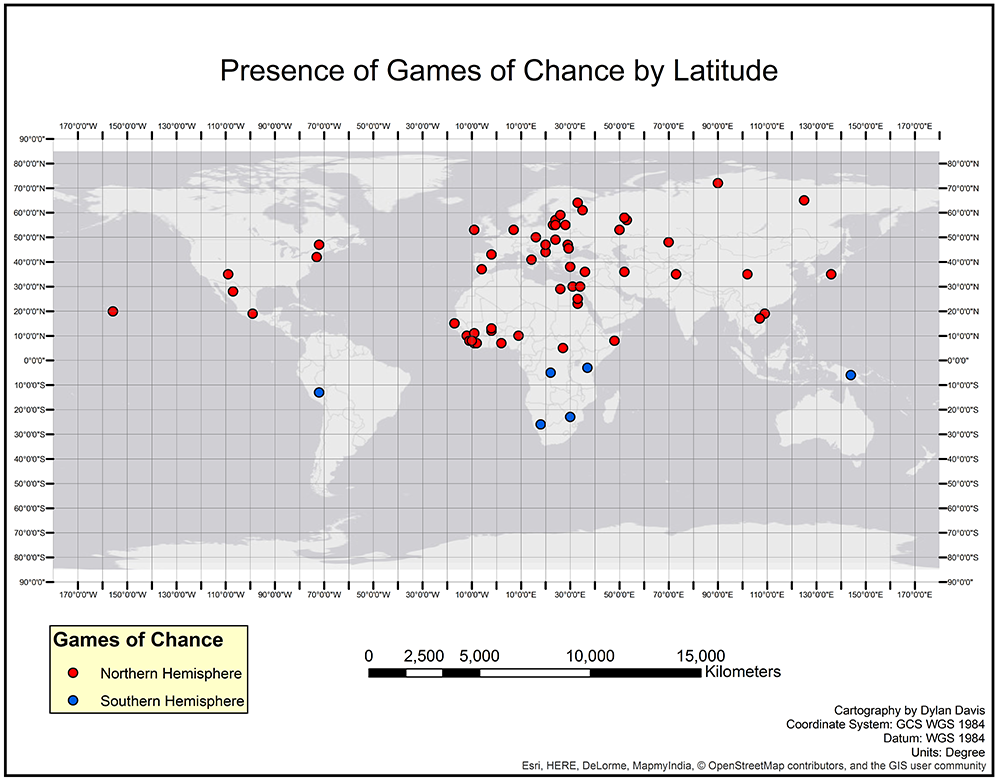
\includegraphics[width=\linewidth]{figures/Figure4_Davis_082016}
	\caption
	\centering
	\label{fig:Figure4_Davis_082016}
\end{figure}

\IJSRAsection{Discussion}

This study has four separate enquiries (Q1-Q4), three of which (Q1-Q3) test (either directly or indirectly) different hypotheses proposed by \textcite{roberts1959}. In particular, it is the goal of this study to retest Roberts and colleagues hypothesis that games of chance are related to religious systems, which was unable to be directly confirmed by later studies \parencites[e.g.][]{ball1972}{chick1998}. In fact, little attempt has actually been made to replicate this particular hypothesis of Roberts and colleagues \parencite[18]{binde2005}. Part of the reason for this lack of re-visitation is the low reliability of the data used by \textcite{roberts1959} and the very small sample size \parencite[18]{binde2005}. Despite these limitations, I address the hypothesis utilising a sample size of 377 cultural groups, and test the hypothesis on the basis of the presence of ``moralistic High Gods”, which is similar to a test conducted by \textcite{ball1972}. 

I determine that games of chance are correlated with the presence of ``High Gods” that are ``moralistic” – meaning that the gods are active and supportive of human morality and are involved in the everyday lives of human beings (Q1). This statistical relationship is statistically significant, meaning that the correlation found by \textcite{ball1972}, as well as the results of the study by \textcite{roberts1959}\footnote{\textcite{roberts1959} use a different set of variables for their study. They compare the prevalence of benevolent, aggressive, and coercive gods and their relation to the presence of games of chance. This study tries to bridge the gap between Roberts et al.’s variables and the presence of ``moralistic” gods, asserting that moralistic gods are benevolent to those that follow moral guidelines and are aggressive towards those that do not follow moral guidelines. As a result, in the presence of ``moralistic” gods, benevolence should be at a higher level than with a lack of such deities.}  appear to be more than mere coincidence. This means that the presence of games of chance is linked to the presence of moralistic gods, which can be considered to be ``benevolent” (as hypothesised by Roberts and colleagues). For further illustration, I conducted a kernel density test on the data, which shows overlap between areas with the presence of ``High Gods” and games of chance (see \cref{fig:Figure5_Davis_082016}). On this note, it can also be stated that in many cultures, games of chance, especially gambling, have been associated with spiritual/supernatural power \parencite[22]{binde2005}[147]{binde2007}.

\begin{figure} [!htb] %FIGURE 5
	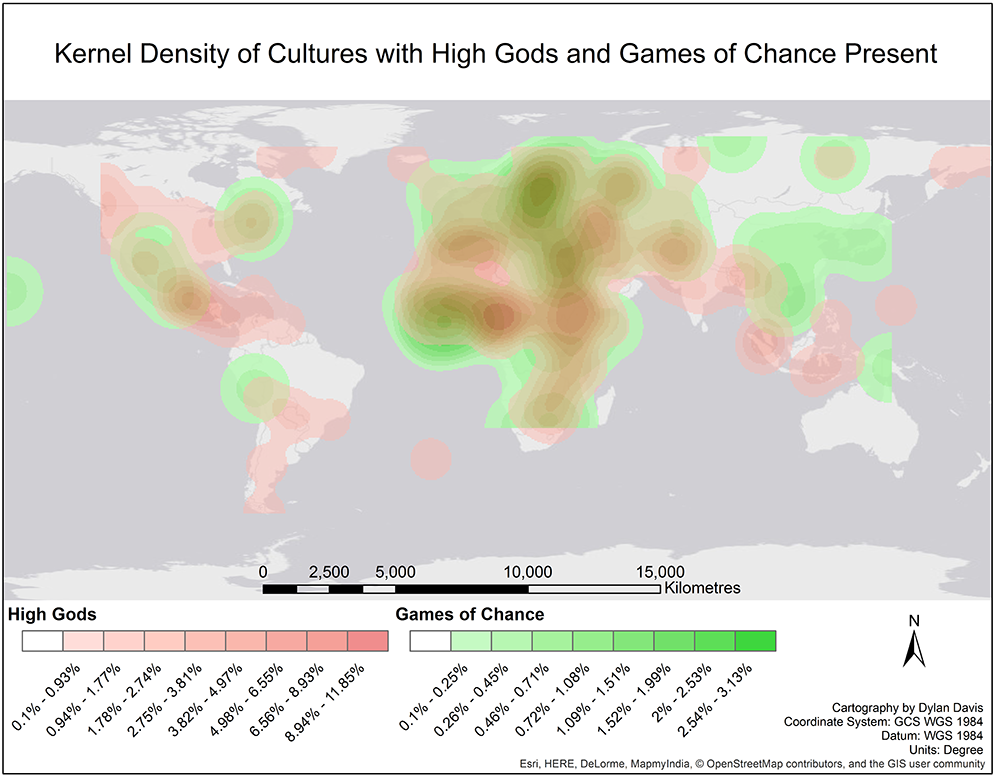
\includegraphics[width=\linewidth]{figures/Figure5_Davis_082016}
	\caption
	\centering
	\label{fig:Figure5_Davis_082016}
\end{figure}

One of the primary reasons for a correlation between religion and games of chance is the concept of illusory control \parencites[see][]{wohl2002}{langer1975}. As stated by \textcite[312]{langer1975}: 
%%%EMBEDDED QUOTE
The belief that everyone gets what he deserves denies the operation of chance. It eliminates the necessity for concern and worry over the possibility that aversive events may occur by chance at any time. Events become predictable and thus, by being anticipated, are often controllable.
%%%EMBEDDED QUOTE
\textcite[323]{langer1975} goes on to state that ``The greatest satisfaction or feeling of competence” will ``result from being able to control the seemingly uncontrollable.” According to the concept of illusory control, individuals desire control over most (if not all) aspects of life, and will thus find some way in which to gain control over a situation. The possession of power has been found to lead to illusory control – or a state of perceived control over the outcome of certain situations \parencite{fast2009}. As a result, those that believe in supernatural powers will be more likely to develop correlations between chance and divine intervention, thereby developing a sense of illusory control in such situations in order to control the outcomes of such games \parencite[1089]{tobacyk1991}.

Looking at the results of Q2, I find that there is no statistically significant relationship between trance states and possession and the presence of games of chance. What this means is that although the presence of gods that intervene in human affairs is correlated with games of chance, the intervention on behalf of the supernatural to influence the outcome of a game is not statistically relevant to the presence of chance games. This result suggests that the presence of a ``moralistic” god instils a set of morals indicating right and wrong, and thereby offers guidelines for what constitutes individuals who are ‘good’ and those that are ‘bad’. Furthermore, for individuals who are deemed ‘bad’ by their god(s), it is suggested that punishment will befall them, and benefits will come to those who are deemed ‘good’. Therefore, although direct intervention is unrelated to the presence of games of chance, the belief in some type of karma or consequence for one’s actions can be said to be related to the presence of chance games. On this point, \textcite{robinson2015} asserts that:
%%%EMBEDDED QUOTE
The common game of Snakes and Ladders originated in India and the early boards were adorned with Hindu gods. The random elements of the game had their roots in Karma and the player's fortune was seen as being determined not as a random act but by fate. In Ancient Egypt these random elements may have been seen as the destiny of the gods also, as being governed by the universal truth of Maat.
%%%EMBEDDED QUOTE
Thus, games of chance – like the game of Snakes and Ladders – in India and Egypt were rooted in beliefs in fate and divine intervention, thereby highlighting the interconnectivity between religious beliefs and the popularity of games of chance.

It must be understood that a connection between material culture and religion is not unexpected. Religion is but a set of ideals, whereas ritual constructs a tangible relationship between those ideals and extant social systems \parencite[14]{bell1992}. As such, material entities are a crux to the existence and success of a religious system. Material objects allow people to ``participate in the divine and to use religion as a technology to manage the beyond of the world in which we live” \parencite[99]{hodder2016}. Games are one such means to an end. 

Relating the results of Q1 and Q2 to \textcite{roberts1959}, it can be affirmed that the belief in gods who are benevolent (i.e. moralistic and deal reward as well as punishment) is statistically related to the presence of games of chance. However, direct aid by the supernatural – which is used by \textcite[602]{roberts1959} as a justification for their results – cannot be said to be true. Nonetheless, religion and games of chance do appear to be correlated, thus reaffirming the results of Roberts and colleagues.

Additional evidence in support of these conclusions comes from the archaeological site of Vijayanagara in southern India. Within this city were many palaces, temples, and shrines, and in association with these features many game-boards were discovered, engraved within stone on or near these architectural structures \parencite[462-463]{rogersdotter2015}. \textcite{rogersdotter2015} classifies the different game-boards found at Vijayanagara into six different categories: alignment games, hunt games, war games, race games, mancala games, and unspecified game types. Of these classes, race games were based on chance, relying on the rolling of dice or throwing of sticks. Consequently, \textcite{rogersdotter2015} finds that race games were the most abundant game type found within the site of Vijayanagara. Additionally, as a major city with a large and socio-economically diverse population, Vijayanagara possessed a large number of the six different types of game boards, consisting of games of chance and strategy. 

In Ancient Egypt particularly (but many other areas as well), the games of \textit{senet} and \textit{mehen} were often played in social contexts, particularly during funerals \parencite[34]{kendall2007}. Both \textit{senet} and \textit{mehen} are considered ``race games”, whereby the objective is to reach a certain point on the game-board and usually includes some type of randomizing agent such as dice \parencite[3]{gobet2004}. In \textit{senet}, casting sticks and \textit{astragali} (knucklebones) were often used (rather than dice) and the game itself became entangled with funerary rites and religious ritual \parencites{piccione1980}[58]{piccione2007}. \textit{Senet} came to be viewed as an activity that bridged the gap between the dead and the living, whereby the game itself acted as a method of communication between the two worlds \parencites[59]{piccione2007}{robinson2015}. Additionally, \textit{mehen} was often found in similar contexts to \textit{senet}, and was also linked with the afterlife \parencite[40-41]{kendall2007}. Both of these games have been found with the context of tombs, signaling their connection to death and journey to the afterlife. Another game similar to \textit{mehen}, called the ``Hyena Game” appeared after \textit{mehen} lost popularity and too comprised a multitude of cosmological motifs \parencite[44]{kendall2007}. Both \textit{mehen} and the ``Hyena Game” contain the same ritualistic meaning, as described by \textcite[44]{kendall2007}: ``the first player to exit the board may well have been thought actually to become \textit{Mehen}, so that the small lion [game] pieces may have been conceptualized as the instruments by which the snake [the board was constructed in the shape of a snake] could destroy the ‘enemies of \textit{Re}’.” As such, games such as \textit{senet}, \textit{mehen}, and offshoots such as the ``Hyena Game” are metaphysical constructs between the realms of the living and the dead, and as such are often recovered in funerary contexts (i.e. tombs). These games are chance based, and therefore illustrate how religious beliefs can affect the types of games played, and the contexts in which those games are played. 

One final example illustrating the connection between religion and games of chance comes from the Zuni culture. Zuni (or Zu\~{n}i) is a Native American group located in the Southwest of the United States. The Zuni possessed all three major game types – strategy, physical skill, and chance (see Appendix \cref{fig:Davis-Table06a} and \cref{fig:Davis-Table06b}). Games like \textit{sh\'{o}liwe} (a gambling game involving arrow reeds) were said to have originated with the Zuni Gods of War, and was then passed to the Zuni people by their mythical ancestors \parencite[480]{stevenson1903}. The game itself is played ceremonially to induce rain, but can also be played outside of this realm as a normal gambling activity \parencite[480]{stevenson1903}. Thus, \textit{sh\'{o}liwe} is rooted in religious beliefs, but also contains a secular nature. Additionally from \textit{sh\'{o}liwe}, other games revolving around chance also existed, some of which were also linked to mythology and religion \parencite{stevenson1903}. 

The next enquiry (Q3) was devoted to looking at political complexity and their relations to the presence of different game types. The results of a cross-cultural comparison of 331 different cultural groups reveal a correlation between population size and the number of different game types present. This result was not unexpected, due to the repeated conclusion that political complexity is related to a more complex series of games and a larger number of game types \parencites[291]{ball1972}[322]{chick1984}[195]{chick1998}{chick2015}{peregrine2008}{roberts1959}. In addition to this test, comparison between political integration level was compared to the presence of strategy games in order to retest another hypothesis established by \textcite{roberts1959} and retested by \textcite{chick1998}, but this time with a larger sample size ($n = 183$). The results once again reaffirm that games of strategy are related to higher levels of political integration.\footnote{This is also supported by evidence from Vijayanagara \parencite{rogersdotter2015}}.

The last area of investigation in this paper is separate from the \textcite{roberts1959} study, and looks at geographical differences for the distribution of game types (Q4). The results indicate that games of chance are overwhelmingly abundant in the northern hemisphere. This result was then compared to mean community population sizes and the presence or absence of ``moralistic” gods. What was determined is that in almost all of the cultural groups included in the sample ($n = 377$) that had games of chance ($n = 63$), 90.5\% (57 out of 63) of them have either moralistic gods or gods that intervene in human affairs (see \cref{fig:Figure6_Davis_082016}). Additionally, in the areas that had such deities present, most had mean community population sizes of at least 50,000 persons (see \cref{fig:Figure7_Davis_082016}). Conclusions that can be drawn from these spatial patterns are that chance and religion are correlated, and religion and population size are correlated. Therefore, religion and population size are correlated, and the presence of games of chance (like all game types) is related to the population level present in a group. The fact that the majority of cultures possessing ``moralistic” gods and games of chance are located in the northern hemisphere is linked to the fact that the vast majority of large population centres are located in the northern hemisphere.

There are a number of variables which influence where people establish themselves and how they develop. Especially important in regards to the establishment of different cultural groups are environmental variables. In a study conducted by \textcite{botero2014}, it is determined that populations possessing a belief in moralising high gods are more prevalent in areas that are at exposed to greater levels of ecological pressure. \textcite[16786]{botero2014} examine 583 cultural groups and determine that the belief in moralistic high gods is directly correlated to political complexity, spatial proximity to other cultures that believe in such deities, ecological variables, the presence of animal husbandry and agriculture, and linguistic origins. This sheds some light on why the distribution of religious systems is uneven: they are linked to a plethora of other factors, including the environment.\footnote{For a detailed discussion of the relationship between religion and environmental factors, \textcite{davis}. In particular, Davis argues that religious systems can reinforce environmentally conscious practices, and such religious ideologies can influence innovation and the use of resources.} Furthermore, due to the fact that game types are related to the religious beliefs present, they too are related to population size, political complexity, technology, and ecological factors present in an area. Therefore, environmental differences may have some effect on the game types present in a given cultural group. One should be critical of generalisations however, and further studies should be undertaken to confirm or dismiss such a claim.

\begin{figure} [!htb] %FIGURE 6
	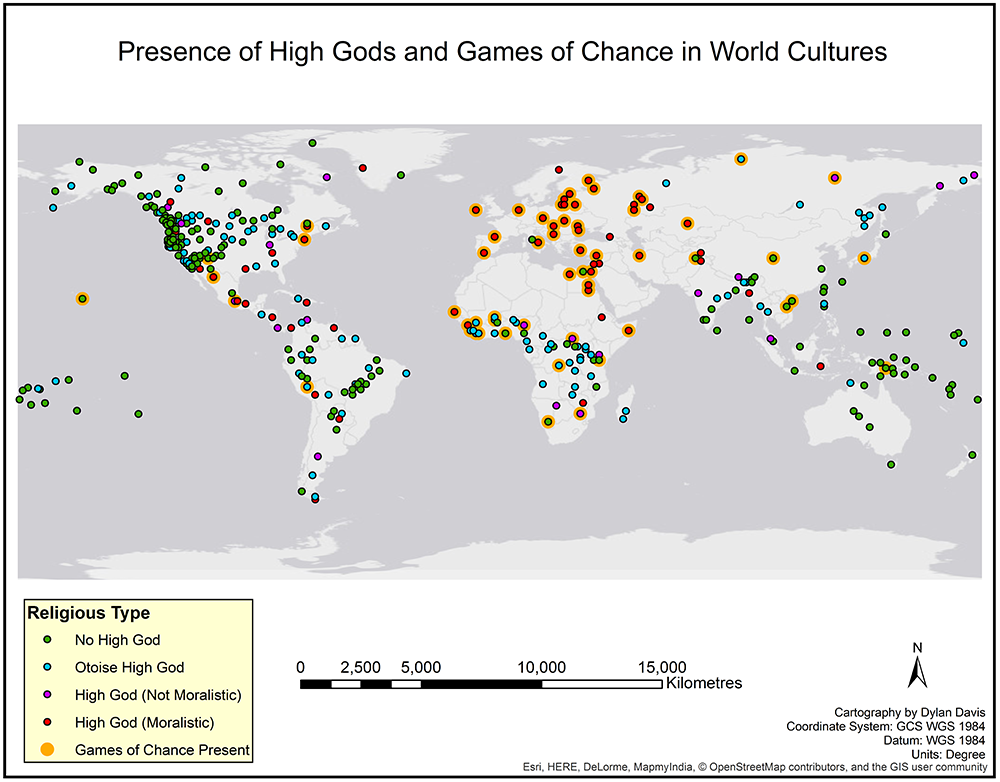
\includegraphics[width=\linewidth]{figures/Figure6_Davis_082016}
	\caption
	\centering
	\label{fig:Figure6_Davis_082016}
\end{figure}

\begin{figure} [!htb] %FIGURE 7
	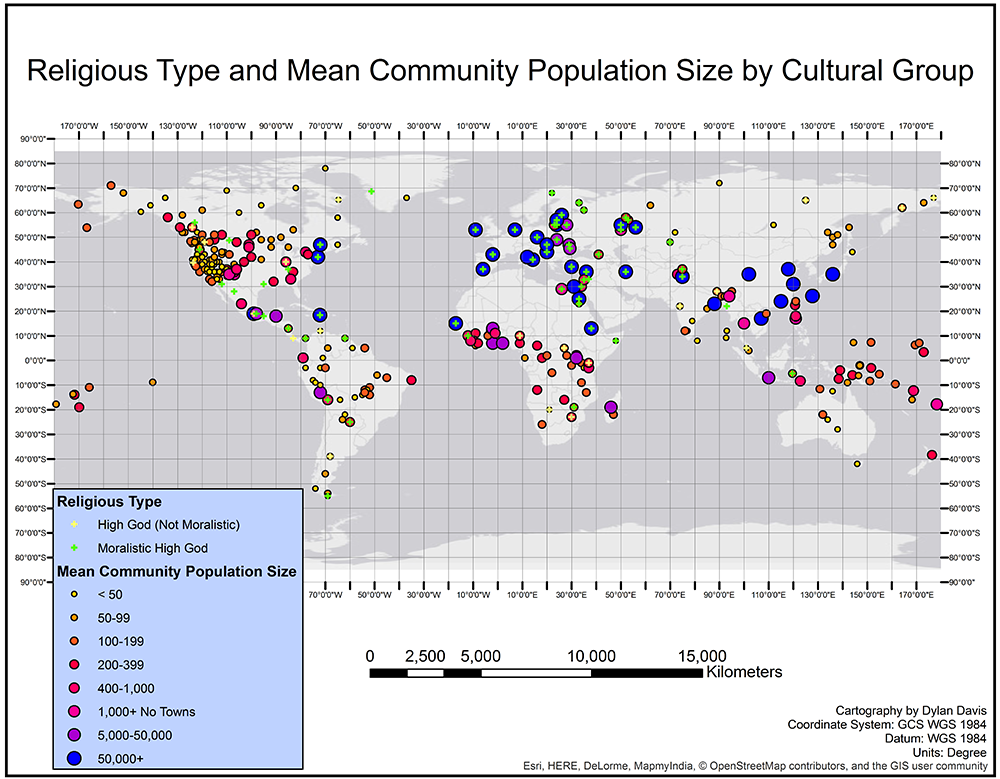
\includegraphics[width=\linewidth]{figures/Figure7_Davis_082016}
	\caption
	\centering
	\label{fig:Figure7_Davis_082016}
\end{figure}

\IJSRAsection{Conclusion}

Cross-cultural comparisons have long been undertaken, and have oftentimes been severely limited in their sample sizes due to an inability to access data, or a lack of data altogether. Using a new database of cultural variables \parencite{D-PLACE} a re-visitation of one of the most influential cross-cultural analyses of gaming \parencite{roberts1959} is carried out to retest the almost 60 year old hypotheses. In particular, attention is placed on Roberts and colleagues’ hypothesis about games of chance and religion. The results of this study indicate that the presence of games of chance is correlated with the presence of benevolent ``moralistic” gods, therefore reaffirming Roberts and colleagues’ hypothesis. However, the presence of a belief in supernatural intervention (i.e. possession of people or objects) shows no relation to the presence or absence of chance games. The belief in divine intervention was used by \textcite[601-602]{roberts1959} as a justification for a linkage between religion and chance games, but has been invalidated by this study. Additionally, other aspects of the \textcite{roberts1959} study are reinvestigated, particularly the relation between game types and socio-political complexity. All components of the Roberts et al. study – minus a link between divine intervention and chance games – appear to be valid.

For archaeologists, these conclusions reaffirm that games, especially games of chance, possess ritual importance and can be linked to ritualistic activities. Additionally, the presence of games in an archaeological site can suggest about the area’s population size, religious system, and political integration level. The use of online databases (like D-PLACE) also has important benefits to archaeologists, who can now compare certain elements of archaeological cultures with other cultural groups in the same geographic region, or across the globe, allowing for a global comparison of the archaeological record. Such studies can enlighten us about human nature, cultural diffusion patterns, and the diversity of humans, as well as their similarities, throughout the globe.

Separate from retesting old conclusions, a cross-cultural investigation into the presence of certain types of games in relation to latitude was conducted, revealing that the northern hemisphere has more variety, and a greater number of cultural groups that possess games of chance, as well as religious systems with ``moralistic” gods. The reasoning for this spatial patterning is left to be explored, but should be the focus of future anthropological research. Correlations between gods, games, and geography exist across cultures, and can give important insights for archaeologists, anthropologists, and social scientists in general.



\IJSRAclosing%<---- don’t change this!
\end{document}